\documentclass[11pt]{article}

%%%%%%%%%%%%%%Include Packages%%%%%%%%%%%%%%%%%%%%%%%%%%
\usepackage{xcolor}
\usepackage{mathtools}
\usepackage[a4paper, total={6in, 8in}, margin=1.25in]{geometry}
\usepackage{amsmath}
\usepackage{amssymb}
\usepackage{paralist}
\usepackage{rsfso}
\usepackage{amsthm}
\usepackage{wasysym}
\usepackage[inline]{enumitem}   
\usepackage{hyperref}
\usepackage{tocloft}
\usepackage{titlesec}
\usepackage{colortbl}
\usepackage{wrapfig}
\usepackage{pdfpages}
%%%%%%%%%%%%%%%%%%%%%%%%%%%%%%%%%%%%%%%%%%%%%%%%%%%%%%%%



\begin{document}

\begin{wrapfigure}[11]{r}{0.42\textwidth}
  \begin{center}
  \vspace{-15pt}
    \includegraphics[scale=0.85]{hat}
  \end{center}
\end{wrapfigure}
\Large \noindent \textbf{Physics 5A Discussion (Week 9)}\\
\normalsize
Department of Physics and Astronomy, UCLA\\
\noindent\rule{8cm}{0.4pt}\\
%\begin{center}
%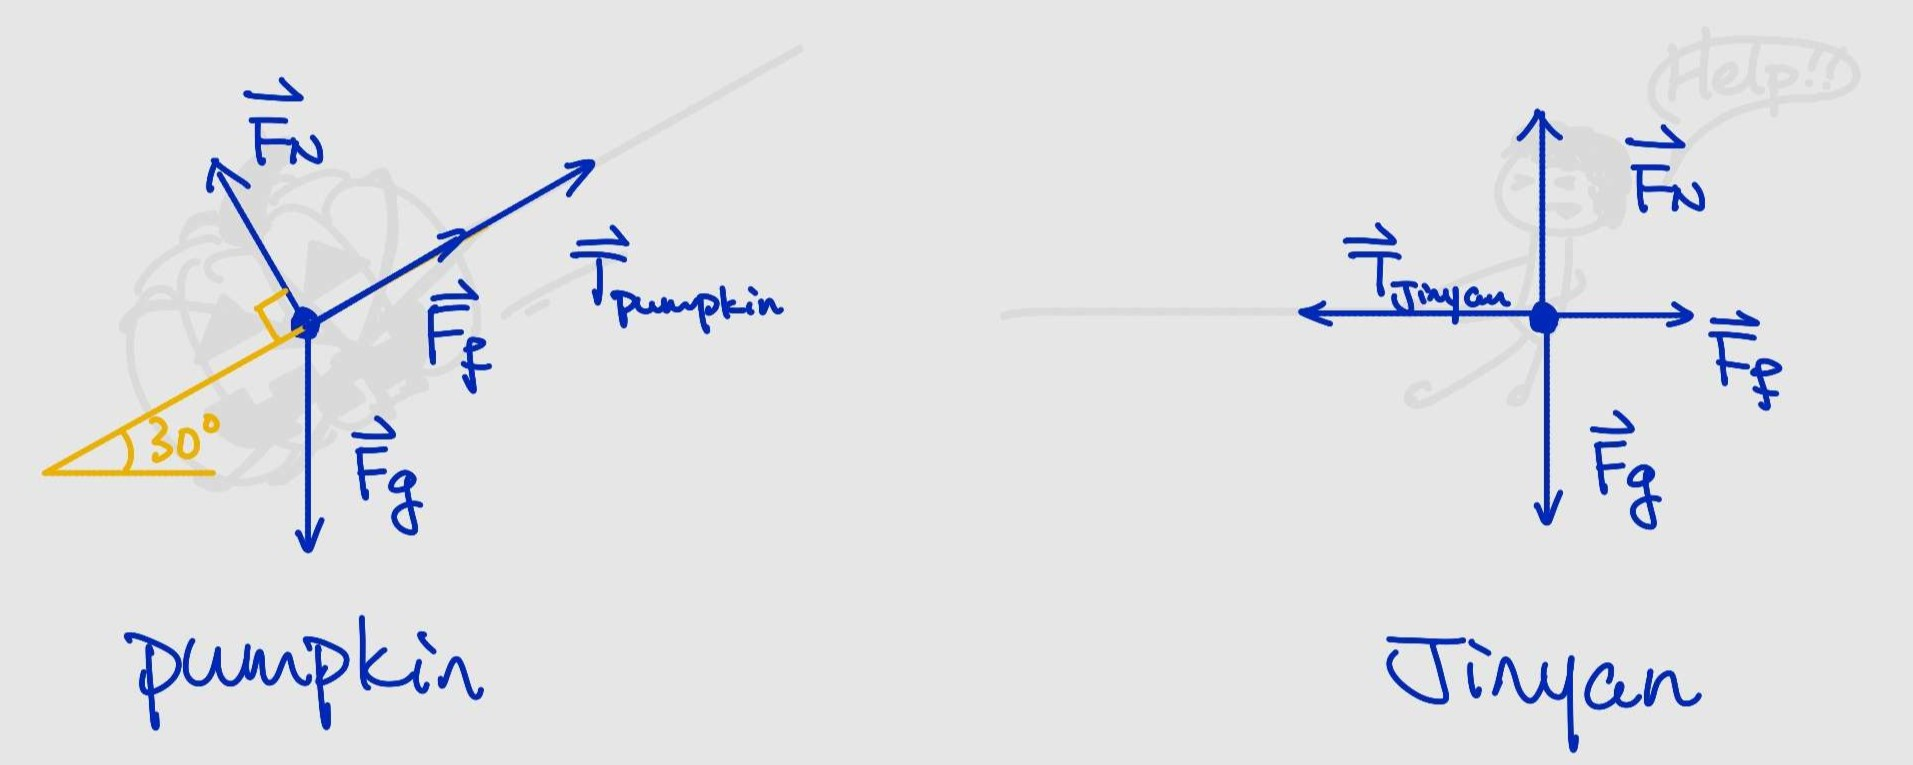
\includegraphics[scale=0.55]{pull}
%\end{center}
Jinyan is climbing a cliff using a rope. At some moment, he reaches a static equilibrium as shown, with his body being parallel to the ground. Jinyan is $1.7\,$m tall and has a mass of $60\,$kg. The coefficient of static friction of the cliff is $\mu_s = 0.5$. Find the force of tension by the rope acting on Jinyan, and the force by the cliff acting on Jinyan. Assume that the center of mass of Jinyan is at the very center of his body. \\
\hfill\break

\noindent\textit{Hints to solve the problem}:\\
(1) What are the forces acting on Jinyan? \\
(2) Where do those forces apply to Jinyan?\\
(3) Jinyan is not moving, so we need $\vec{F}_{\text{net}}=0$ and $\tau_{\text{net}} = 0$. \\
(4) Draw the free-body diagram, using it to write $\vec{F}_{\text{net}} = m\vec{a} = 0$.\\
(5) Which of those forces is trying to make Jinyan rotate? Use them to write $\tau_{\text{net}} = 0$.\\

\noindent From (4) and (5), you should obtain a set of equations that you can solve for all the unknown forces. \\

\newpage
\textbf{Solution to the problem}:
To solve this problem, we first ask what are the forces that we need to consider here. (a) The first thing that we should consider is gravitational force, and it acts at the center of mass of Jinyan. (b) Since Jinyan's foot is stepping on the cliff wall, the cliff wall provides a normal force, preventing Jinyan from going through the wall. The normal force should be perpendicular to the surface, acting on the point of contact. (c) Friction comes into play: the static friction by the cliff wall is preventing Jinyan from sliding up or down, also acting at the point of contact. (d) Since Jinyan is holding a rope, tension acts at Jinyan's hand.\\

Summarizing (a), (b), (c), and (d), we have the following diagram, including all forces acting on Jinyan.
\begin{center}
\includegraphics[scale=0.65]{rotate}
\end{center}


Now, all forces need to be considered when applying Newton's second law, which is 
\begin{align*}
0 = m \vec{a} = \vec{F}_{\text{net}} = \vec{F}_{g} + \vec{F}_N + \vec{F}_f + \vec{F}_T\,.
\end{align*}
Writing out the component form, we have
\begin{align*}
&\text{$x$-direction:\ }0 = 0 + (-F_N) + 0 + F_T \cos(\theta)\,.\\
&\text{$y$-direction:\ }0 = (-mg) + 0 + F_f + F_T \sin(\theta)\,.\\ 
\end{align*}
The notation here assumes $F_N,\ mg,\ F_f,\ F_T$ to be positive. \textbf{Important note}: Here $F_f \neq \mu_s\, F_N$ because we are talking about static friction, not kinetic friction. \\

Jinyan is not rotating, to determine which forces would make Jinyan rotate, we first need to choose a pivot point, which is the point that Jinyan would rotate around. For simplicity, we choose the pivot point at the point where Jinyan's foot is touching the cliff wall. Forces acting at the pivot point do not contribute to the rotation (\textbf{fact}), so normal force and friction do not contribute any torque. Gravitational force and tension force do contribute torques. The torque by the gravitational force is
\begin{align*}
\tau_{g} =\text{("force")}\cdot \text{("distance")} =(mg)\cdot (d/2)
\end{align*}
where $d=1.7$ m is Jinyan's height. This is because the gravitational force is acting at Jinyan's center of mass, right at the middle of Jinyan's body, $d/2$ distance away from the pivot, being perpendicular to Jinyan's body. Next, the torque by the tension is 
\begin{align*}
\tau_T =\text{("force")}\cdot \text{("distance")} = (-F_T \sin(\theta)) \cdot (r)
\end{align*}  
where $r=1$ m is the distance from the pivot to Jinyan's hand, and $\theta$ is the angle between the direction of $\vec{F}_T$ and Jinyan's body. We need to use $\sin(\theta)$ here to extract the component of $\vec{F}_T$ that is perpendicular to Jinyan's body. \\

We take counterclockwise rotation to be positive. Gravitational force is trying to make Jinyan rotate counterclockwise around the pivot and thus $\tau_g$ is expected to be positive. However, the tension is trying to make Jinyan to rotate clockwise, thus $\tau_T$ is expected to be negative. \\

Now the net torque is zero because Jinyan is not rotating, so
\begin{align*}
0=\tau_{\text{net}} = \tau_g + \tau_T = \frac{mgd}{2} - F_T\sin(\theta)\,r\,.
\end{align*}
Combining everything we have discussed so far, we obtain three equations for three unknowns, $F_N$, $F_f$, and $F_T$,
\begin{align*}
\begin{cases}
0 = -F_N + F_T \cos(\theta)\\
0= -mg + F_f + F_T \sin(\theta)\\
0 = mgd/2 - F_T \sin(\theta)\, r\end{cases}\ .
\end{align*}
All other variables in these equations, $\theta,\ m,\ g,\ d,$ and $r$ are given in the problem. Plugging in all the numbers, we have
\begin{align*}
\begin{cases}
0 = -F_N + F_T \cos(30^\circ)\\
0= -(60\cdot 9.8) + F_f + F_T \sin(30^\circ)\\
0 =  (60\cdot 9.8\cdot 1.7/2) - F_T \sin(30^\circ) \cdot 1
\end{cases}\ .
\end{align*} 
Using your favorite method for solving a system of equations (for instance, we can use the third equation to solve for $F_T$ first, then use the second one to solve for $F_f$, and lastly the first one to solve for $F_N$), we obtain 
\begin{align*}
F_T = 1000\,\text{N}\,,\qquad
F_N = 865\,\text{N}\,,\qquad
F_f = 88.2\,\text{N}\,.
\end{align*}
For a consistency check, we should verify that $F_f < \mu_s F_N = 432.5\,\text{N}$, such that static friction applies. Thus the force by the cliff acting on Jinyan is the normal force $F_N = 865$\,N and the friction force $F_f = 88.2$\,N. 


\end{document}


